\section{Static Program Analysis and Evidence Generation Engine}
\label{sec:engine}

The operational core of Reg2App translates abstract program properties into concrete static inspection routines. The prototype engine accepts production Android packages, systematically deconstructs their Dalvik bytecode and resources, and synthesizes an Evidence Provenance Graph $G = (V, E)$ (Figure~\ref{fig:system_architecture}).

\begin{figure*}[t]
\centering
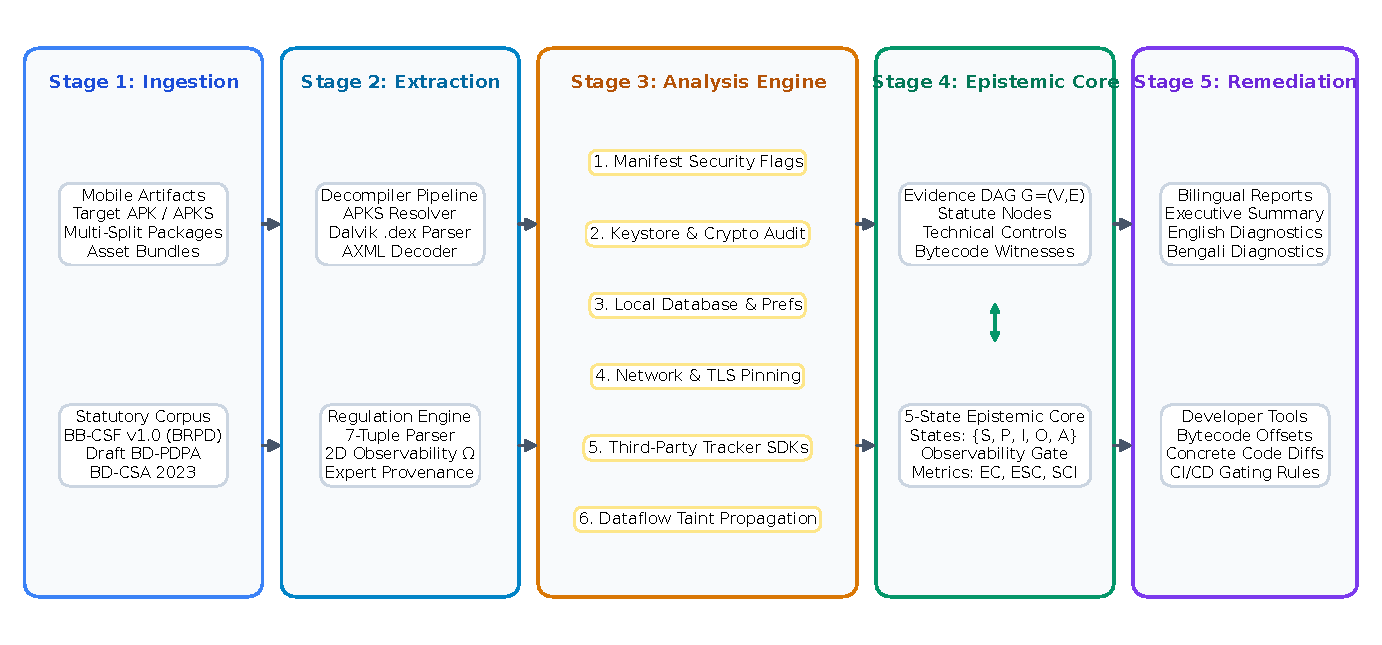
\includegraphics[width=0.78\textwidth]{figures/fig2_system_architecture.pdf}
\caption{\textbf{The Reg2App System Architecture}: Static analysis and evidence generation pipeline. Application archives (\texttt{.apk} and multi-split \texttt{.apks}) are ingested alongside declarative Regulation-as-Code YAML knowledge bases. The extraction pipeline disassembles Dalvik bytecode and decodes binary XML resources. Six decoupled static analysis modules evaluate specific program properties, emitting evidence witnesses into the tiered Evidence Provenance Graph $G = (V, E)$. The 5-State Epistemic Evaluator computes objective metrics ($EC, ESC, SCI$) and feeds the localized reporting engine to generate actionable English and Bengali diagnostics.}
\label{fig:system_architecture}
\end{figure*}

\subsection{Extraction and Decompilation Pipeline}
\label{sec:engine:extraction}

Modern Android applications are distributed as monolithic APKs or multi-split App Bundles (\texttt{.apks}). As implemented in \texttt{reg2app/analyzers/apk\_extractor.py}, Reg2App resolves both formats across three sequential phases:
(1)~\textit{Bundle Resolution}: Extracts the primary \texttt{base-master.apk} containing the core manifest and Dalvik bytecode (\texttt{classes.dex}), while aggregating architecture-specific configuration splits (\texttt{config.arm64\_v8a.apk}) and resource splits.
(2)~\textit{Bytecode Disassembly}: Integrates Androguard~\cite{androguard} to parse Dalvik bytecode across Multi-Dex distributions ($\text{classes.dex}, \dots, \text{classes}N\text{.dex}$), extracting complete method call graphs, field references, and string constants into an internal AST representation.
(3)~\textit{Binary Resource Decoding}: Decodes binary AXML resources, including \texttt{AndroidManifest.xml} and \texttt{res/xml/network\_security\_config.xml}, into structural DOM objects.

\subsection{Modular Static Program Analyzers}
\label{sec:engine:analyzers}

Reg2App orchestrates six specialized, decoupled static analysis modules:

\paragraph{1) Manifest Security Analyzer} Inspects declarative security configurations in \texttt{AndroidManifest.xml}: verifies whether \texttt{android:allowBackup="false"} (preventing ADB data extraction under BB-CSF §4.1.5.21); flags \texttt{android:debuggable="true"} (allowing arbitrary runtime memory inspection); evaluates \texttt{android:usesCleartextTraffic}; and identifies exported components lacking explicit permissions (CSA §17).

\paragraph{2) Cryptographic Misuse Analyzer} Following the empirical taxonomy of Egele et al.~\cite{crypto_misuse_ccs} and CogniCrypt~\cite{cognicrypt}, this module inspects invocations of \texttt{javax.crypto} and \texttt{java.security}. It parses transformation strings passed to \texttt{Cipher.getInstance()}, flagging electronic codebook (ECB) modes while requiring authenticated modes (AES-GCM) under BB-CSF §4.1.5.19. It identifies hardcoded static keys in string pools (BB-CSF §4.1.5.18), verifies hardware-backed key generation via \texttt{KeyGenParameterSpec.Builder} with \texttt{AndroidKeyStore}~\cite{ekberg_tee}, and flags predictable pseudorandom number generators.

\paragraph{3) Storage Protection Analyzer} Evaluates persistence mechanisms against PDPA §15 and BB-CSF §4.1.5.21: detects plaintext \texttt{SharedPreferences} and verifies migration to \texttt{EncryptedSharedPreferences}; examines \texttt{SQLiteOpenHelper} calls for SQLCipher integration; and flags storage writes to world-readable external directories (\texttt{getExternalStorageDirectory()}).

\paragraph{4) Network Security Analyzer} Audits communications against BB-CSF §4.1.3.12 and CSA §21: parses \texttt{network\_security\_config.xml} for cleartext traffic bans, valid \texttt{\textless{}pin-set\textgreater{}} SHA-256 hashes on payment endpoints, and certificate expiration; and flags empty \texttt{checkServerTrusted()} methods or non-validating \texttt{HostnameVerifier} implementations~\cite{fahl_msc, castle_crypto}.

\paragraph{5) Third-Party SDK and Tracker Analyzer} Scans namespaces and classpaths against signature registries of analytics, advertising, and tracking SDKs (e.g., AppsFlyer, Facebook, Adjust, Firebase)~\cite{leontiadis_sdk, binns_third_party_trackers}, identifying undeclared background telemetry exfiltration under PDPA §§23 and 28.

\paragraph{6) Dataflow Taint Tracking Engine} Adapts inter-procedural taint propagation from FlowDroid~\cite{flowdroid, amandroid, iccta}, tracking flows from sensitive sources (device IDs, GPS, user input) to untrusted sinks (network sockets, logs, unencrypted storage).

\subsection{Resilience to Obfuscation, Reflection, and Packing}
\label{sec:engine:obfuscation}

Reg2App handles adversarial transformations through disciplined design:
(1)~\textit{Identifier Renaming (ProGuard/R8)}: Because Reg2App targets invocations of immutable Android framework and Java APIs (e.g., \texttt{javax.crypto.Cipher}, \texttt{AndroidKeyStore}), system-level method signatures cannot be renamed by compilers, ensuring AST call-graph matching remains robust against identifier mangling.
(2)~\textit{Dynamic Reflection and String Encryption}: When applications invoke APIs reflectively (e.g., \texttt{Class.forName()}) or decrypt arguments at runtime, static AST traversal cannot resolve immediate string arguments~\cite{octeau_reflection, ernst_static_dynamic}. Rather than emitting speculative verdicts, Reg2App's decision function $\mathcal{D}$ returns $\bot$, transitioning the requirement to $\mathbf{InsufficientEvidence}$ and alerting auditors.
(3)~\textit{Dex Packing}: When applications employ commercial packers that encrypt bytecode into native stubs, Reg2App flags the APK as packed based on DEX headers and native library signatures, emitting an explicit requirement for dynamic memory dumping prior to verification.
(4)~\textit{Native JNI}: When banking apps delegate cryptography to compiled C/C++ libraries (\texttt{.so}), Reg2App isolates these boundaries as $\mathbf{InsufficientEvidence}$ rather than assuming compliance.

\subsection{The Evidence Provenance Graph \texorpdfstring{($G$)}{(G)}}
\label{sec:engine:graph}

To provide verifiable forensic traceability, Reg2App synthesizes analysis outputs into a directed acyclic graph $G = (V, E)$, where $V$ partitions into four semantic tiers:
\begin{equation}
V = V_{\text{Statute}} \cup V_{\text{Control}} \cup V_{\text{Property}} \cup V_{\text{Witness}}
\end{equation}
Here, $v_s \in V_{\text{Statute}}$ represents a statutory article (e.g., \texttt{BB-CSF-4.1.3.12}); $v_c \in V_{\text{Control}}$ represents the technical control (e.g., \texttt{CTRL-NET-01}); $v_p \in V_{\text{Property}}$ represents the observable program property; and $v_w \in V_{\text{Witness}}$ represents the concrete evidence witness (cryptographic hash, bytecode offset, XML snippet). The edge set $E$ models provenance derivation:
\begin{equation}
E = E_{\text{normative}} \cup E_{\text{operational}} \cup E_{\text{observational}}
\end{equation}
When an auditor queries why a clause is evaluated as $\mathbf{PotentialNonConformance}$, Reg2App executes a reverse topological traversal from $v_s$ through $E$, retrieving the exact witness $v_w$ (e.g., class \texttt{CryptoUtil}, method \texttt{encrypt()}, offset 84, \texttt{Cipher.getInstance("AES/ECB")}), providing complete auditability.
